\documentclass[10pt,twocolumn,letterpaper]{article}

\usepackage{cvpr}
\usepackage{times}
\usepackage{epsfig}
\usepackage{graphicx}
\usepackage{amsmath}
\usepackage{amssymb}
\usepackage[utf8]{inputenc}
\usepackage{listings}
\usepackage{color}
\usepackage{graphicx}
\graphicspath{ {images/} }

% Include other packages here, before hyperref.

% If you comment hyperref and then uncomment it, you should delete
% egpaper.aux before re-running latex.  (Or just hit 'q' on the first latex
% run, let it finish, and you should be clear).
\usepackage[breaklinks=true,bookmarks=false]{hyperref}

\cvprfinalcopy % *** Uncomment this line for the final submission

\def\cvprPaperID{****} % *** Enter the CVPR Paper ID here
\def\httilde{\mbox{\tt\raisebox{-.5ex}{\symbol{126}}}}

% Pages are numbered in submission mode, and unnumbered in camera-ready
%\ifcvprfinal\pagestyle{empty}\fi
\setcounter{page}{1}
\begin{document}

%%%%%%%%% TITLE
\title{PHOW Classification}

\author{Juan Sebasti\'an D\'iaz\\
201127333\\
Universidad de los Andes\\
{\tt\small js.diaz1591@uniandes.edu.co}
% For a paper whose authors are all at the same institution,
% omit the following lines up until the closing ``}''.
% Additional authors and addresses can be added with ``\and'',
% just like the second author.
% To save space, use either the email address or home page, not both
\and
Juli\'an Alexander Martinez\\
201213994\\
Universidad de los andes\\
{\tt\small ja.martinez1423@uniandes.edu.co}
}

\maketitle
%\thispagestyle{empty}

%%%%%%%%% ABSTRACT
\begin{abstract}
   In this practice, PHOW techniques are used to recognize elements in in image. The imagenet database is used and the MATLAB  functions of CALTECH 101  are used. these functions obtained 92\% accuracy in the latter database and it is to find out the accuracy in IMAGENET.
\end{abstract}
%%%%%%%%% BODY TEXT

\section{Image-Net Database}

ImageNet came after PASCAL VOC, in the need of having an image database rich in categories and in day-to-day images. This database contains 996 categories with 100 images each, presenting the object in different scales and positions, all of the images being natural images. IMAGENET is organized in a hierarchy of "synonym sets", which are concepts described by multiple words and are later subdivided to make a more fine classification. These synonym sets come from WordNet, where there are more that 100,000 synonym sets or "synsets". IMAGENET was built upon WordNet, and was meant to describe each synset with at least 1000 images.

\begin{figure}[h]
\begin{center}
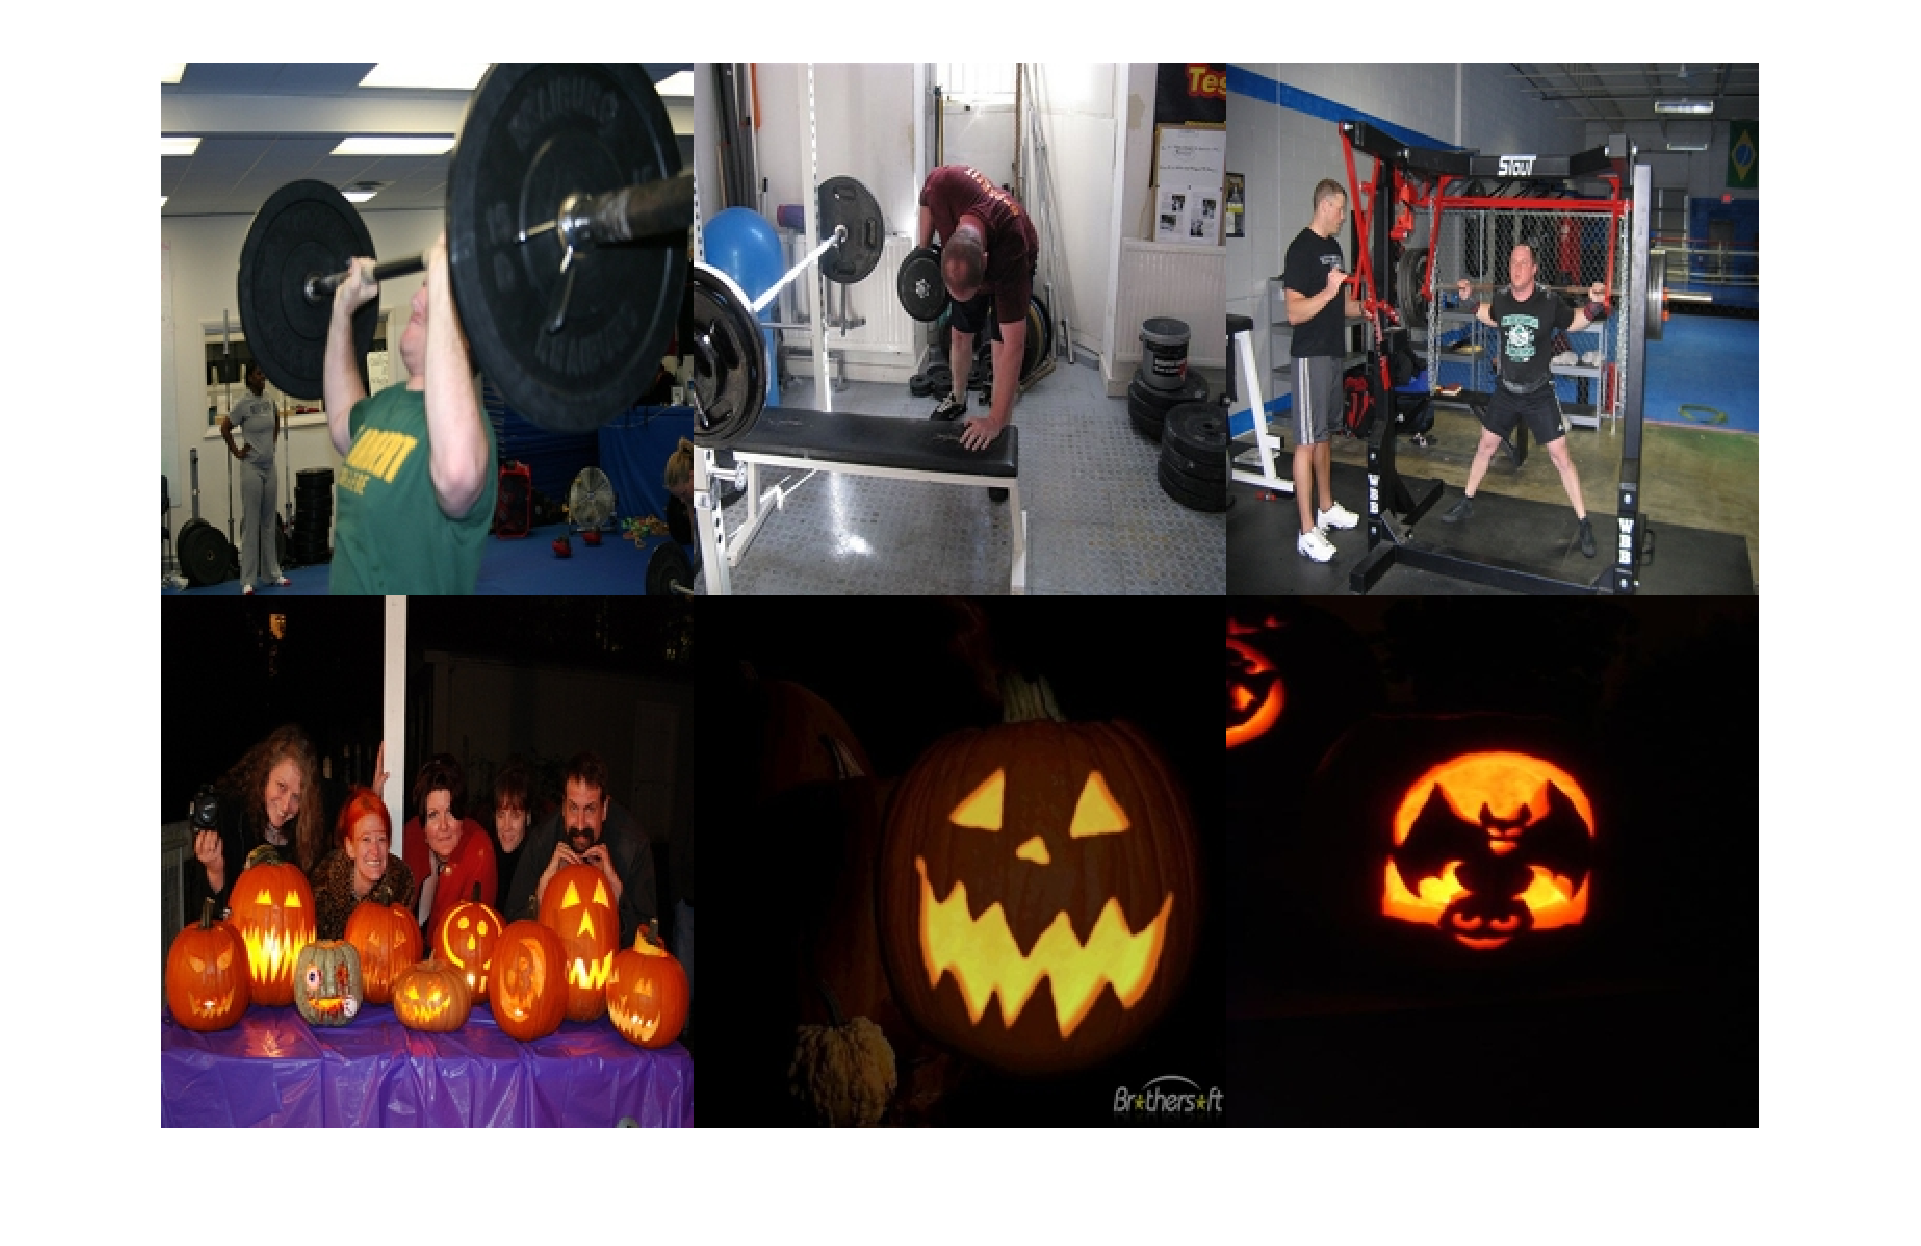
\includegraphics[width=1\linewidth]{images/DataBase.eps}
\end{center}
   \caption{
This is an example of the classes and the picture that composed the data based IMAGENET
   }
\label{DataBase}
\end{figure}
%------------------------------------------------------------------------
\section{Recognition Methods}

The method used for recognition was PHOW (dense SIFT descriptors) that used a similar organization as the texton classification. The code used was obtained from the VLFeat group, which has an open source of computer vision algorithms. First, PHOW descriptors were obtained from some train images. Thae database of train was huge, so some samples of the database of different sizes were chosen to see the performance of the method. These are the \textit{words}. These words are clustered using \textit{k-means} to find the dictionary (as with the texton dictionary), or \textit{bag of words}. Using this bag of words, the train set (or sample of the set) of images is represented using the clusters found on the latter step. The images and their respective representation is then used to train a SVM. The test images used to evaluate the model are also represented with the bag of words, so they can be correctly represented by the SVM just trained. 


%-------------------------------------------------------------------------
\section{Results}

The results shown in this section was obtained in the train section of the data base. At the beginning it was expected that this results was only the validation set of our model, but eventually after a lot of time ruining the algorithm obtaining this results; it was decided to assume this experiments as the result of the model. This was possible assuming either the train set as the test set was balanced and working in one of them only limit the number of images in order to train the SVM. Another important specification was that all the models was tested with 20 images.

The result of the proposed algorithm yields two graphs, as shown in Figure \ref{baseline-result}:

\begin{figure}[h]
\begin{center}
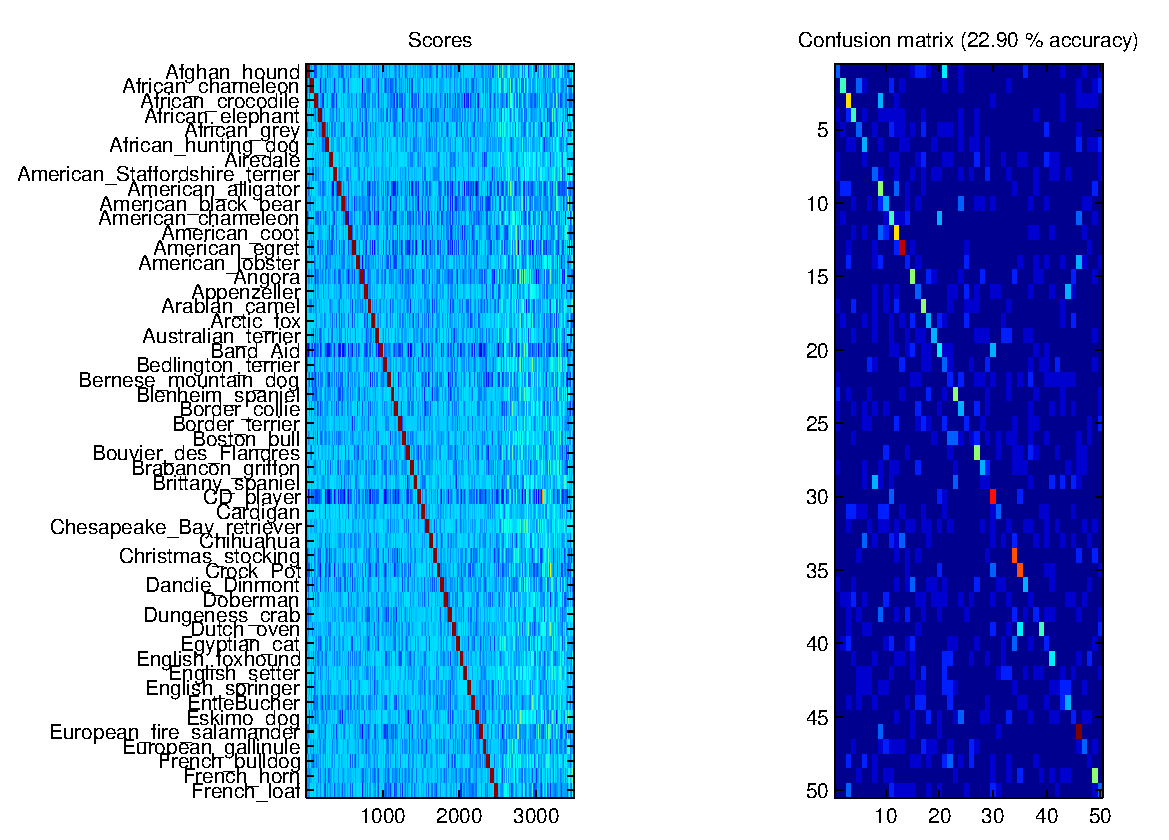
\includegraphics[width=1\linewidth]{images/baseline-result.eps}
\end{center}
   \caption{
Matrix of scores and confusion matrix generated by the code. This shown  the results of the algorithm after train and test the models obtained.
   }
\label{baseline-result}
\end{figure}

The graph on the right corresponds to the confusion matrix, where red corresponds to a high and blue low. Ideally in this case it is expected to have completely red diagonal matrix with completely blue outside of  it. The points outside the diagonal correspond to misclassifications, contributing to error. The two axes correspond to the categories.

\begin{figure}[h]
\begin{center}
\includegraphics[width=1\linewidth]{images/nTrain1.eps}
\end{center}
   \caption{
Accuracy obtained varying the number of images in train stage. The following parameters was fixed: Number of words = 600, Spatial partition = [2 4], Parameter C SVM = 10, Number of Class = 5, PHOG descriptor = 1.
   }
\label{nTrain1}
\end{figure}

The graph on the left corresponds to \textit{score} that gives the classifier to the classification of each evaluated image. The color scale is the same as in the graph to the right. When an image has a dark red dot on this graph, it means that the classifier is quite sure which class belongs. The horizontal axis corresponds to each of the evaluated images and the vertical axis to the classes they belong.

\begin{figure}[h]
\begin{center}
\includegraphics[width=1\linewidth]{images/nClass1.eps}
\end{center}
   \caption{
Accuracy obtained varying the number of classes to identify. The following parameters was fixed: Number of words = 600, Spatial partition = [2 4], Parameter C SVM = 10, Number of train images = 50, PHOG descriptor = 1.
   }
\label{nClass1}
\end{figure}

The work focused primarily on the effect of variation of different parameters in training and classification of images.The accuracy and the time required to train and classify images by varying number of categories, number of training images and number of space partitions was measured.

\begin{figure}[h]
\begin{center}
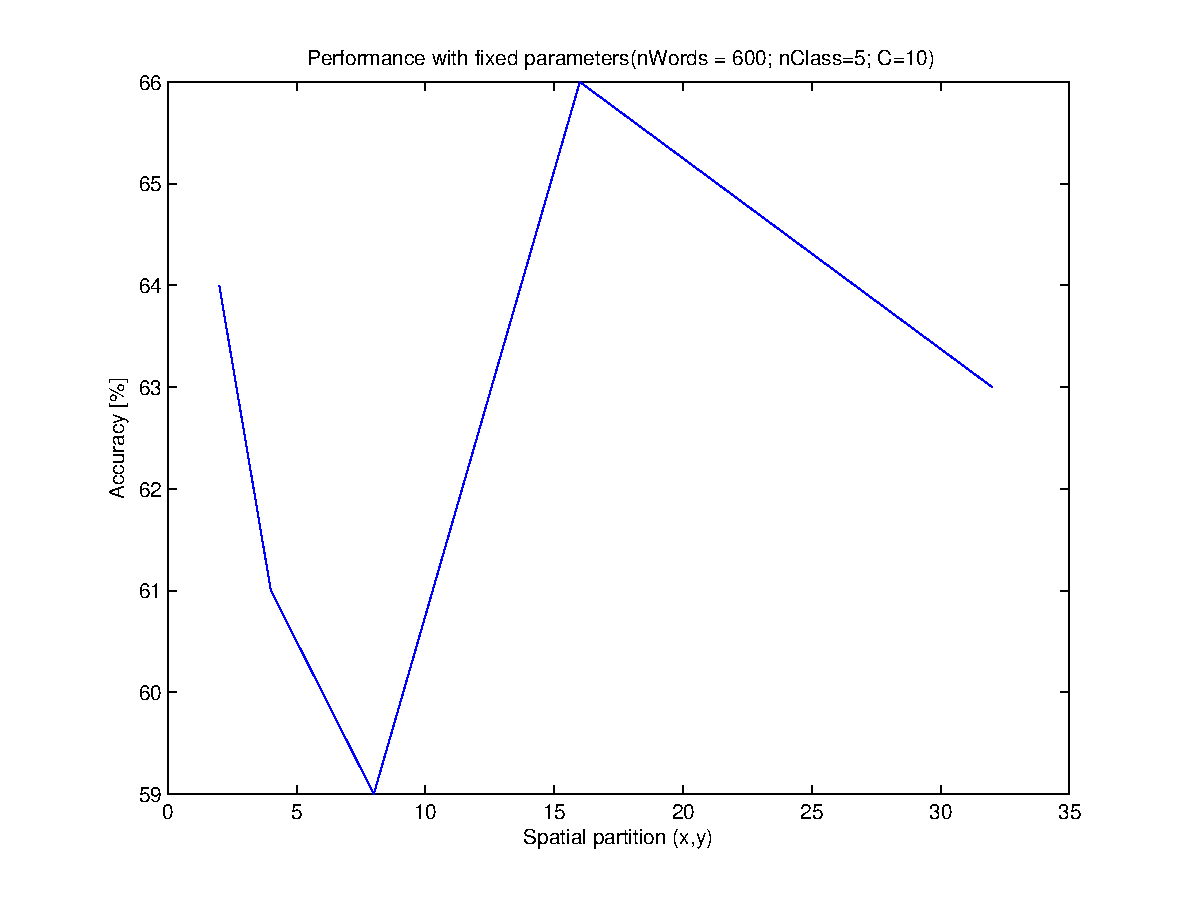
\includegraphics[width=1\linewidth]{images/nSpatial1.eps}
\end{center}
   \caption{
Accuracy obtained varying the number spatial partition. The following parameters was fixed: Number of words = 600, Number of Classes = 5, Parameter C SVM = 10, Number of train images = 50, PHOG descriptor = 1.
It is important to say that the number 16 and 32 in the x-axe represent spatial partitions of [2 4] and [2 8].
   }
\label{nSpatial1}
\end{figure}

According to the above, the results of accuracy by varying the number of classes, the number of training images and spatial partition are in Figures \ref{nClass1}, \ref{nTrain1} and \ref{nSpatial1} respectively.

\begin{figure}[h]
\begin{center}
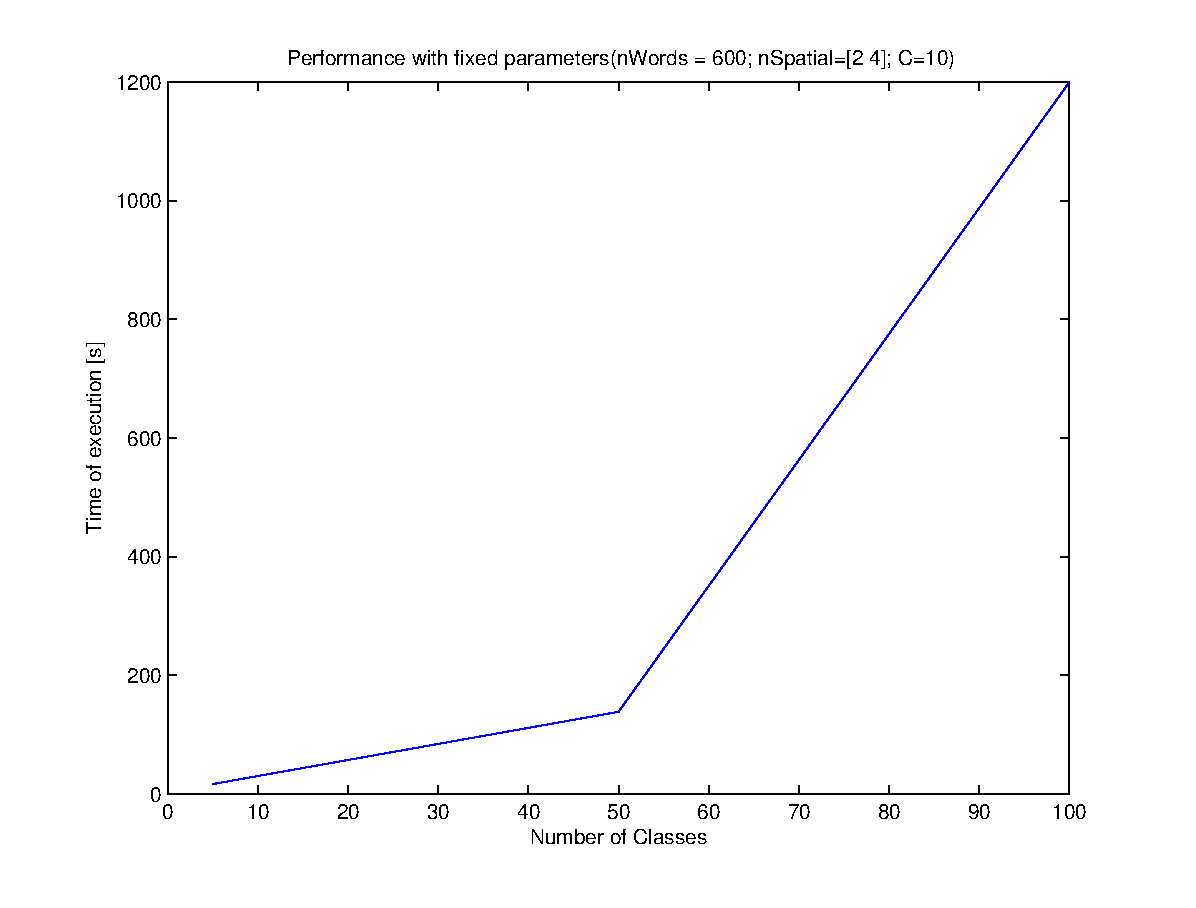
\includegraphics[width=1\linewidth]{images/nClass2.eps}
\end{center}
   \caption{
Time elapse in each of the experiments varying the number classes to identify. The following parameters was fixed: Number of words = 600, spatial partition = [2 4], Parameter C SVM = 10, Number of train images = 50, PHOG descriptor = 1.
   }
\label{nClass2}
\end{figure}

The evaluation of computational resources required for each case was done by measuring the time required to perform each of the training and evaluations. These times for variation in the number of classesand spatial partition are in Figures \ref{nClass2} and \ref{nSpatial2} respectively.

\begin{figure}[h]
\begin{center}
\includegraphics[width=1\linewidth]{images/nSpatial2.eps}
\end{center}
   \caption{
Time elapse in each of the experiments varying the number spatial partitions. The following parameters was fixed: Number of words = 600, Number of classes = 5, Parameter C SVM = 10, Number of train images = 50, PHOG descriptor = 1.
   }
\label{nSpatial2}
\end{figure}

However as it is described in each of the Figures above there are some other parameters fixed in the analysis of each one. For that reason, and trying to get a better understand of the hole model these fixed parameters was also running in the algorithm making changes in their values. It is important to mentioned that the PHOG parameter has only two values 0 and 1 in order to codify a group of parameters configurations. In the case of 0 the step of the sliding window was 3 and the other was establish by default. In the case of 1 the step was set in 5 and the size of the window set in 7. These two configurations was decided because they were in the code of Caltech 101, the 0 option was the tiny configurtion and the 1 option was the complete problem. In these way it was expected to have a more detailed descriptor in the 0 option than in the 1 option. These parameters that was analysed in addition was the numbers of words, the parameter C of the margin in the SVM and the configurations of the PHOG.

\begin{figure}[h]
\begin{center}
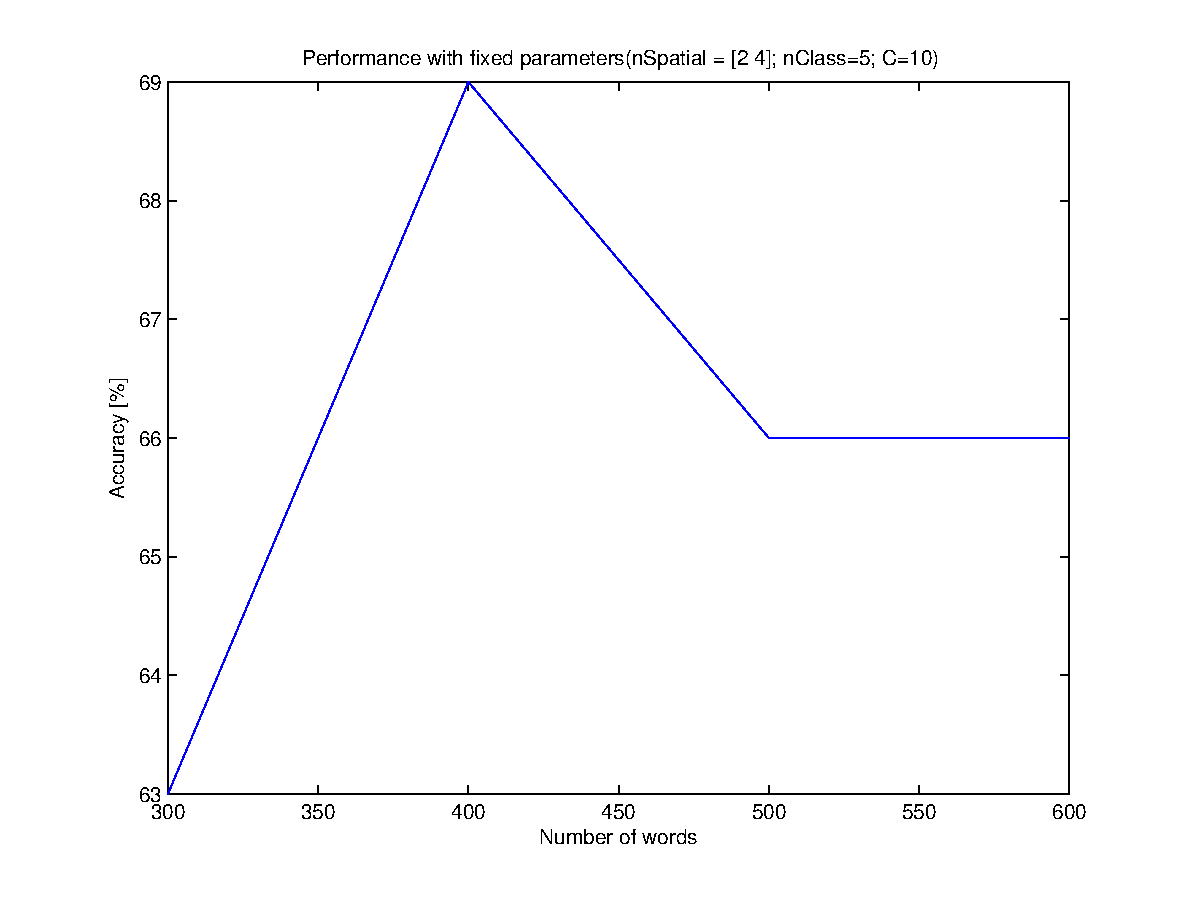
\includegraphics[width=1\linewidth]{images/nWords1.eps}
\end{center}
   \caption{
Accuracy obtained varying the number of words. The following parameters was fixed: Number of Classes = 5, Spatial partition = [2 4], Parameter C SVM = 10, Number of train images = 50, PHOG descriptor = 1.
   }
\label{nWords1}
\end{figure}

According to the above, the results of accuracy by varying the number of words, the parameters of PHOW and the C margin of SVM are in Figures \ref{nWords1}, \ref{C1} and \ref{pHOG1} respectively.

\begin{figure}[h]
\begin{center}
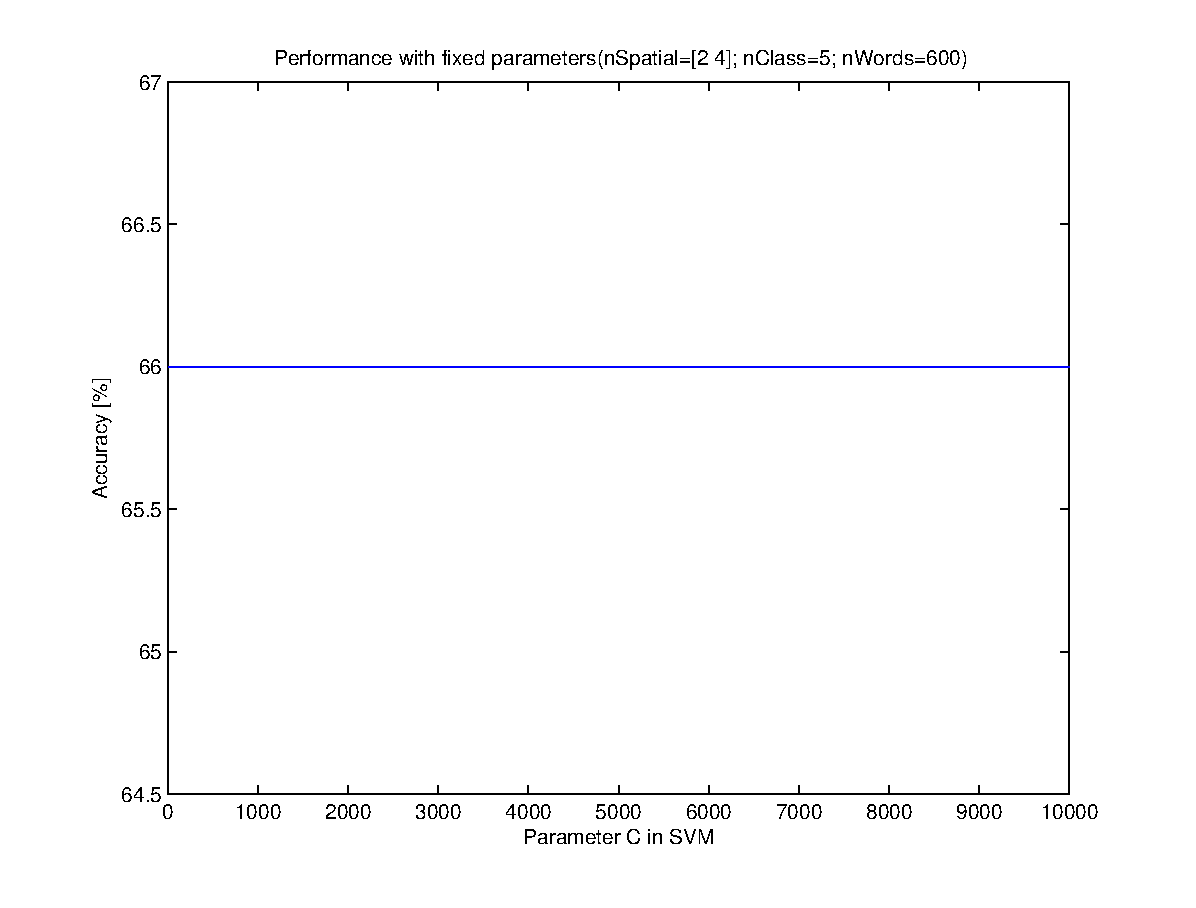
\includegraphics[width=1\linewidth]{images/C1.eps}
\end{center}
   \caption{
Accuracy obtained varying margin C of SVM. The following parameters was fixed: Number of Words = 600, Spatial partition = [2 4], Number of Classes = 5, Number of train images = 50, PHOG descriptor = 1.
   }
\label{C1}
\end{figure}

The evaluation of computational resources required for the additional cases was done by measuring the time required to perform each of the training and evaluations. These times for variation in the number of words , the margin C and the configuration of pHOW are in Figures \ref{nWords2} ,\ref{C2} and \ref{pHOG2} respectively.

\begin{figure}[h]
\begin{center}
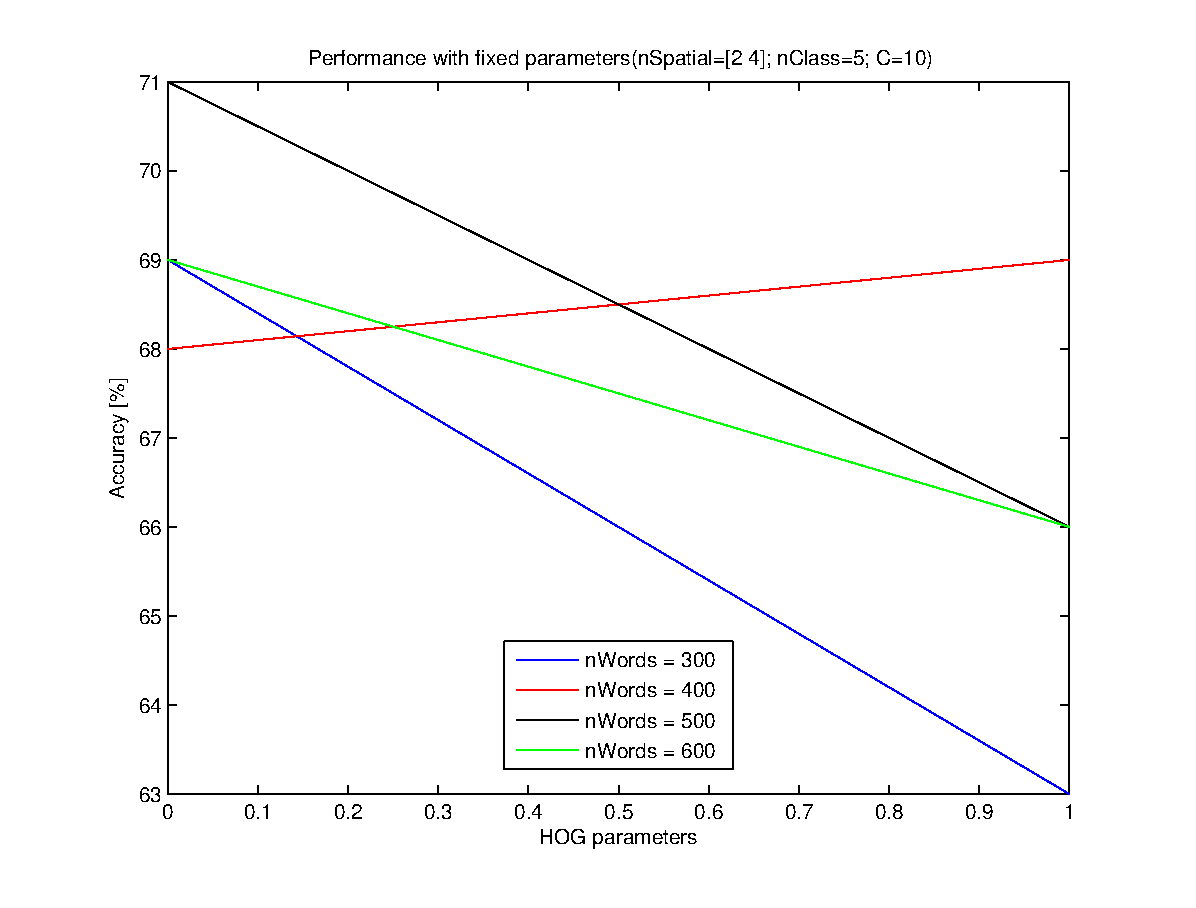
\includegraphics[width=1\linewidth]{images/pHOG1.eps}
\end{center}
   \caption{
Accuracy obtained varying the configuration of the HOG descriptor. The following parameters was fixed: Number of Words = 600, Spatial partition = [2 4], Number of Classes = 5, Number of train images = 50, Parameter C SVM = 10.
   }
\label{pHOG1}
\end{figure}

\begin{figure}[h]
\begin{center}
\includegraphics[width=1\linewidth]{images/nWords2.eps}
\end{center}
   \caption{
Time elapse in each of the experiments varying the number of words. The following parameters was fixed: Spatial partition = [2 4], Number of classes = 5, Parameter C SVM = 10, Number of train images = 50, PHOG descriptor = 1.
   }
\label{nWords2}
\end{figure}

\begin{figure}[h]
\begin{center}
\includegraphics[width=1\linewidth]{images/C2.eps}
\end{center}
   \caption{
Time elapse in each of the experiments varying the margin parameter C. The following parameters was fixed: Number of words = 600, Number of classes = 5, Spatial partition = [2 4], Number of train images = 50, PHOG descriptor = 1.
   }
\label{C2}
\end{figure}

\begin{figure}[h]
\begin{center}
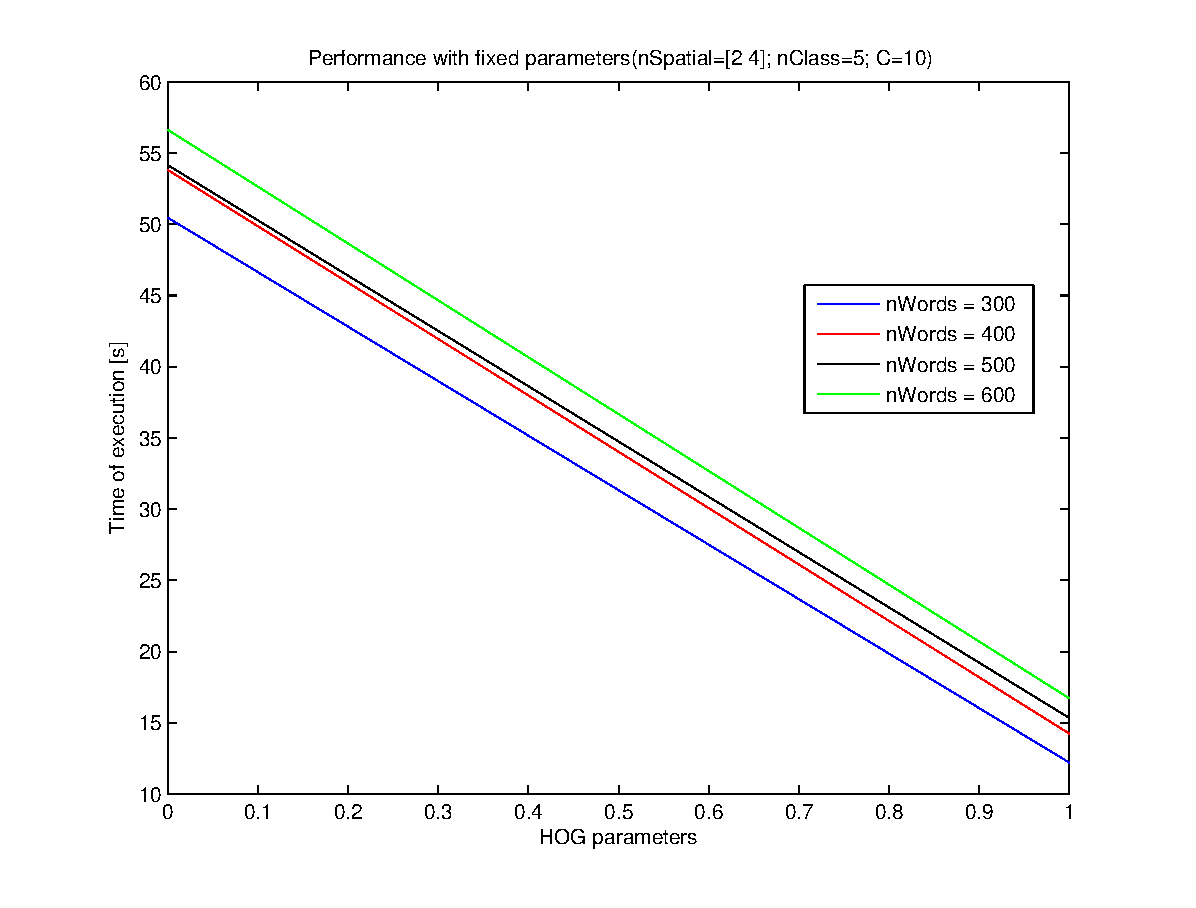
\includegraphics[width=1\linewidth]{images/pHOG2.eps}
\end{center}
   \caption{
Time elapse in each of the experiments varying the HOG configuration. The following parameters was fixed: Number of words = 600, Number of classes = 5, Parameter C SVM = 10, Number of train images = 50, Spatial partition = [2 4].
   }
\label{pHOG2}
\end{figure}

%-------------------------------------------------------------------------
\section{Discussion of the results}

The results of the algorithm in the data base are not the best one because the architecture was design in order to original applied the MATLAB routine in the Caltech 101 data base, and because of the different range of difficulties in the two data base the phow\_caltech101 algorithm had not a good performance on IMAGENET. However as an special case when the algorithm has the parameters in the table \ref{SpecialCase} it has an accuracy of 75\% but only in the 0.005\% of the categories of all the data base. 

\begin{table}[h]
\centering
\begin{tabular}{|l|l|l|l|l|l|}
\hline
nTrain & nClass & nWords & nSpatial & C & pHOG
\\ \hline
50 & 5 & 500 & [2 4] & 10 & 1 \\ \hline
\end{tabular}
\caption{Parameters of the case in which the AC was 75\%}
\label{SpecialCase}
\end{table}

The graphs presented above show that there is a dependency between the parameters used in computing resources and performance of classifiers, a detail behaviour of each case is described in the next subsection.

\subsection{Number of categories}

By varying the number of classes, leaving constant the other parameters , you have to build a more complex model including more categories using the same amount of training images per class. This causes a decreased in performance rating of test images, as shown in Figure \ref{nClass1}. As you increase the number of classes, the performance is worse, making more misclassification. The relationship is not linear; instead of it seems to have an exponential decay behavior, where the less categories it has to classify the better accuracy the algorithm obtained. However, the idea of these problems is to correctly classify a lot of categories, so the solution is not to use less of them but modify other parameters or performance space to achieve good results with a lot of class. As a possible correlation if the numbers of images to train grow up the accuracy seems to improve, so as an start the number of train images could be a parameter to change in order to improve the model. 

As for the time required to train and test by varying the number of classes is intuitively understand that the more categories, the model is more complex and therefore more computer effort required to build the classifier, specifically the number of svm increase, because it must train one of each category in order to identify one of them from the other . This is shown in Figure \ref{nClass2}, where as the number of classes increases, the time required increases almost linearly, making it a highly significant situation. However in this experiment the only SVM uses was linear, uses another type of SVM could also have a impact in the time and performance of the algorithm.

\subsection{Size of Training set}

By varying the number of training images, leaving the other parameters constant, there are more images to build the svm model per categories. This means that the more images one has to teach the computer, this can best learn a sorting function improving performance. In Figure \ref{nTrain1} this is evident: as the number of classes increases, performance is better, mistaking least in image classification. The relationship appears to be somewhat linear; rather it seems to have an exponential behavior, improving accuracy if more classes are used. Accordingly, in classification problems always you want to have as much training images as possible.

As for the time required to train and test by varying the number of training images to teach the more data, the computer requires to process more images, making a more complete model. Therefore greater effort of the machine to build the classifier is required. This is expected in the behaviour of the time vs nTrain graph.

\subsection{Number of spatial Partitions}

First is important to recall that the point 16 and 32 in the x-axes of the figure \ref{nSpatial1} and \ref{nSpatial2} correspond to the [2 4] and [2 8] parameter set. In the figure \ref{nSpatial1} it could see that the optimal parameter that improve AC is the [2 4]. This parameter change the quantity of the bins in each of the oriented histogram. The behaviour of this maximal point correspond that if the model has few bins histogram the model is too general but if it has many ones the model is too specific and the correspondence with other elements of the same category is low. 

As for the time required to train and test, not only the accuracy of the classifier was better using (2.4), but the time required was less well, choosing this optimal parameter.

\subsection{Number of Words}

The behaviour of the AC in function of the number of words using in the descriptor is similar as spatial partition; it means that has an optimal value in 500 words, or in other words an maximum. This is shown in the \ref{nWords1}. The explanation of this conduct is similar as in the spatial partition, many words create overfiting and few word wide general models. This repetitive conduct in some way is expected in the descriptor parameters because this features mediate the amount of information in each of the descriptor.

Related to the time elapse is the same as spatial partition. As the model uses more words it require more calculation which implies more computational time. This is evidence in the figure \ref{nWords2}. However the change in the amount of time uses
in the execution of all the algorithm it is important  because a double in the number of words translate in an grow in 41.67\% in computational time, almost a linear relation.

\subsection{Margin parameter C in the SVM}

As we could see in the \ref{C1} the change in the margin C of the SVM has no effect on the AC of the algorithm. This could be a result of the characteristic of the descriptor of each model, it means that the each group has a strong cluster that are sufficient apart from each one in order to not be affect by a considerably margin ranging from 10 to 10000. 

According to the time elapse observe in the figure \ref{C2}, the changes observed in the time are not significant meaning that this parameter has a little impact in the final model.

\subsection{Configuration of the pHOW descriptor}

As the other descriptor features parameters the option 1, means a more detailed parameter. The conduct in the figure \ref{pHOG1} is the result an overfiting of the model. However, it is expected that as the number of categories start to grow up, the more detailed parameter have to be applied in order to get in some way a differentiation characteristic.

According to the time of execution the more detailed the descriptor is the more time the algorithm will use, as is eveidence in the figure \ref{pHOG2}.





%-------------------------------------------------------------------------
\section{Limitations of the method and Possible improvements}

It became clear that the methods used in the code obtained from the VLFeat method, worked perfectly on the CALTECH 101 database, which was a small and exemplar database in which the objects in the images were easily recognized. Now, when using the methods on IMAGENET, the performance decreased considerably, because of the nature of the database. The images are normal images, in which objects appear in day-to-day situations, and issues such as occlusion, change in perspective and position and deformations are common.\\

Also, the databases have huge variations in their sizes. As happened with textons, for matters of computing time, not all the training database was used, only a small fraction, which not always represents correctly the whole database and this lead to mismatches in the test part.\\

To improve the correct classification of the IMAGENET database, it should take into account the flexibility of the objects in this database, in contrast to the objects in CALTECH 101. Definitely there should be used more images, but the descriptors obtained should have a certain degree of flexibility to adapt to the test images. One possible approach is to use the spring model, in which the words are linked by springs in the image, and their separation distance can be compressed or elongated to adapt to the object deformities.

%-------------------------------------------------------------------------

%-------------------------------------------------------------------------
\begin{thebibliography}{9}

\bibitem{IN}
  \emph{IMAGENET},
  Standford Vision Lab,
  in http://image-net.org/index


\bibitem{VLF}
\emph{VLFeat Open Sourcce}
in http://www.vlfeat.org/index.html

\end{thebibliography}




%-------------------------------------------------------------------------


\end{document}
